% Begin the document and set up the style of the document
\documentclass[a4paper]{article}

% Install the required packages for the document 
\usepackage{envmath}
\usepackage{esvect}
\usepackage{graphicx}
\usepackage{gensymb}
\usepackage{tikz}
\usepackage{geometry}
\usepackage{enumitem}
\usepackage{mathtools}
\usepackage{graphicx}
\usepackage{amsmath}
\usepackage{amscd}
\usepackage{amssymb}
\usepackage{amsfonts}
\usepackage{harpoon}
\usepackage{pgf}
\usepackage{tikz}
\usepackage{mathrsfs}
\usepackage{asyalign}
\usepackage{physics}
\usepackage{enumitem}
\usepackage{xhfill}
\usepackage{accents}
\usepackage{cite}
\usepackage{url}
\usepackage[tableposition=top]{caption}
\usepackage{ifthen}
\usepackage[utf8]{inputenc}
\usepackage{tikz-3dplot}
\usetikzlibrary{patterns}
\usetikzlibrary{arrows}


\makeatletter
\renewcommand*\env@matrix[1][*\c@MaxMatrixCols c]{%
  \hskip -\arraycolsep
  \let\@ifnextchar\new@ifnextchar
  \array{#1}}
\makeatother

% Page and style settings
\parskip=8pt
\parindent=0pt
% Right margin
\textwidth=6.25in
% Left margin
\oddsidemargin=0pt
\evensidemargin=0pt
% Bottom margin
\textheight=10in
% Top margin
\topmargin=-0.75in
\baselineskip=11pt
% end of page and other style settings

\renewcommand{\familydefault}{\sfdefault}


% Begin the text of the document
\begin{document}

% Begin the Title Page
\begin{titlepage}

\newcommand{\HRule}{\rule{\linewidth}{0.5mm}} % Defines a new command for the horizontal lines, change thickness here

\center % Center everything on the page
 
\textsc{\LARGE University of Sydney}\\[1.5cm] % Name of your university/college
\textsc{\Large MATH 1902 - Linear Algebra (Advanced)}\\[0.5cm] % Major heading such as course name
\textsc{\large Assignment 2}\\[0.5cm] % Minor heading such as course title

\HRule \\[0.4cm]
{ \huge \bfseries Matrices and Hyper Cubes}\\[0.4cm] % Title of your document
\HRule \\[1.5cm]

\begin{minipage}{0.4\textwidth}
\begin{flushleft} \large
\emph{Author:}
Keegan Gyoery % Your name
\\
\emph{SID:}
470413467
\end{flushleft}
\end{minipage}
~
\begin{minipage}{0.4\textwidth}
\begin{flushright} \large
\emph{Tutor:} 
Edwin J Spark % Tutor's Name
\\
\emph{Semester:}
First
\end{flushright}
\end{minipage}\\[4cm]

{\large \today}\\[3cm] % Date, change the \today to a set date if you want to be precise

\vfill % Fill the rest of the page with whitespace

\end{titlepage}

\pagenumbering{arabic}
%%%%%%%%%%%%%%%%%%%%%%%%%%%
%%%%%%%%%%%%%%%%%%%%%%%%%%%
%%%%%%%%%%%%%%%%%%%%%%%%%%%
%%%%%%%%%%%%%%%%%%%%%%%%%%%

% Begin the document and answering the questions
\begin{enumerate}[label=\textbf{\arabic*.}]
	\item Consider the system of equations $A\textbf{x} = \textbf{b}$

			% Build the initial matrix of the question
			$$
			A =
			\begin{bmatrix*}[r]
				\hspace{1mm} 1 & 2 & -1 & -2 \hspace{1mm}\\
				\hspace{1mm}-2 & 1 & 2 & -1 \hspace{1mm}\\
				\hspace{1mm} -1 & -2 & 1 & 2 \hspace{1mm}\\
				\hspace{1mm} 2 & -1 & -2 & x \hspace{1mm}\\
			\end{bmatrix*}
			,
			\hspace{5mm}
			\textbf{x} = 
			\begin{bmatrix*}[r]
				\hspace{1mm} x_1 \hspace{1mm}\\
				\hspace{1mm} x_2 \hspace{1mm}\\
				\hspace{1mm} x_3 \hspace{1mm}\\
				\hspace{1mm} x_4 \hspace{1mm}\\
			\end{bmatrix*}
			,
			\hspace{5mm}
			\textbf{b} =
			\begin{bmatrix*}[r]
				\hspace{1mm} c \hspace{1mm}\\
				\hspace{1mm} d \hspace{1mm}\\
				\hspace{1mm} e \hspace{1mm}\\
				\hspace{1mm} f \hspace{1mm}\\
			\end{bmatrix*}
			$$

			When the system of equations is solved, we are determining the values of $x_1$, $x_2$, $x_3$, $x_4$ that satisfy the augmented matrix $M = [A|\textbf{b}]$.

			% Begin the list to answer part a and b of question 1 
			\begin{enumerate}

				% Question a answer
				\item In order to solve for the variables $x_1$, $x_2$, $x_3$, $x_4$, we use the augmented matrix $[A|\textbf{b}]$. By reducing the augmented matrix to its reduced row echelon form, we are able to solve for the desired variables in terms of $x$, $c$, $d$, $e$, $f$.

				$$
				% Matrix Step 1
				\begin{bmatrix}[rrrr|r]
					\hspace{1mm} 1 & 2 & -1 & -2 \hspace{1mm} & \hspace{1mm} c \hspace{1mm}\\
					\hspace{1mm}-2 & 1 & 2 & -1 \hspace{1mm} & \hspace{1mm} d \hspace{1mm}\\
					\hspace{1mm} -1 & -2 & 1 & 2 \hspace{1mm} & \hspace{1mm} e \hspace{1mm}\\
					\hspace{1mm} 2 & -1 & -2 & x \hspace{1mm} & \hspace{1mm} f \hspace{1mm}\\
				\end{bmatrix}
				% Row Operation Matrix 1
				\begin{matrix}
					~\\
					~\\
					\xrightarrow{R_3 = R_3 + R_1} \\
					~\\
				\end{matrix}
				% Matrix Step 2
				\begin{bmatrix}[rrrr|r]
					\hspace{1mm} 1 & 2 & -1 & -2 \hspace{1mm} & \hspace{1mm} c \hspace{1mm}\\
					\hspace{1mm}-2 & 1 & 2 & -1 \hspace{1mm} & \hspace{1mm} d \hspace{1mm}\\
					\hspace{1mm} 0 & 0 & 0 & 0 \hspace{1mm} & \hspace{1mm} c + e \hspace{1mm}\\
					\hspace{1mm} 2 & -1 & -2 & x \hspace{1mm} & \hspace{1mm} f \hspace{1mm}\\
				\end{bmatrix}
				$$

				% New Line 
				$$
				% Row Operation Matrix 2
				\begin{matrix}
					~\\
					~\\
					\xrightarrow{R_3 = R_4} \\
					\xrightarrow{R_4 = R_3} \\
				\end{matrix}
				% Matrix Step 3
				\begin{bmatrix}[rrrr|r]
					\hspace{1mm} 1 & 2 & -1 & -2 \hspace{1mm} & \hspace{1mm} c \hspace{1mm}\\
					\hspace{1mm}-2 & 1 & 2 & -1 \hspace{1mm} & \hspace{1mm} d \hspace{1mm}\\
					\hspace{1mm} 2 & -1 & -2 & x \hspace{1mm} & \hspace{1mm} f \hspace{1mm}\\
					\hspace{1mm} 0 & 0 & 0 & 0 \hspace{1mm} & \hspace{1mm} c + e \hspace{1mm}\\
				\end{bmatrix}
				% Row Operation Matrix 3
				\begin{matrix}
					~\\
					~\\
					\xrightarrow{R_3 = R_2 + R_3} \\
					~\\
				\end{matrix}
				% Matrix Step 4
				\begin{bmatrix}[rrrr|r]
					\hspace{1mm} 1 & 2 & -1 & -2 \hspace{1mm} & \hspace{1mm} c \hspace{1mm}\\
					\hspace{1mm}-2 & 1 & 2 & -1 \hspace{1mm} & \hspace{1mm} d \hspace{1mm}\\
					\hspace{1mm} 0 & 0 & 0 & x - 1 \hspace{1mm} & \hspace{1mm} d + f \hspace{1mm}\\
					\hspace{1mm} 0 & 0 & 0 & 0 \hspace{1mm} & \hspace{1mm} c + e \hspace{1mm}\\
				\end{bmatrix}
				$$

				% New Line
				$$
				% Row Operation Matrix 4
				\begin{matrix}
					~\\
					\xrightarrow{R_2 = 2R_1 + R_2} \\
					~\\
					~\\
				\end{matrix}
				% Matrix Step 5
				\begin{bmatrix}[rrrr|r]
					\hspace{1mm} 1 & 2 & -1 & -2 \hspace{1mm} & \hspace{1mm} c \hspace{1mm}\\
					\hspace{1mm} 0 & 5 & 0 & -5 \hspace{1mm} & \hspace{1mm} 2c + d \hspace{1mm}\\
					\hspace{1mm} 0 & 0 & 0 & x - 1 \hspace{1mm} & \hspace{1mm} d + f \hspace{1mm}\\
					\hspace{1mm} 0 & 0 & 0 & 0 \hspace{1mm} & \hspace{1mm} c + e \hspace{1mm}\\
				\end{bmatrix}
				% Row Operation Matrix 5
				\begin{matrix}
					~\\
					\xrightarrow{R_2 = \frac{1}{5}R_2} \\
					~\\
					~\\
				\end{matrix}
				% Matrix Step 6
				\begin{bmatrix}[rrrr|r]
					\hspace{1mm} 1 & 2 & -1 & -2 \hspace{1mm} & \hspace{1mm} c \hspace{1mm}\\
					\hspace{1mm} 0 & 1 & 0 & -1 \hspace{1mm} & \hspace{1mm} \frac{2c + d}{5} \hspace{1mm}\\
					\hspace{1mm} 0 & 0 & 0 & x - 1 \hspace{1mm} & \hspace{1mm} d + f \hspace{1mm}\\
					\hspace{1mm} 0 & 0 & 0 & 0 \hspace{1mm} & \hspace{1mm} c + e \hspace{1mm}\\
				\end{bmatrix}
				$$

				% New Line
				$$
				% Row Operation Matrix 6
				\begin{matrix}
					~\\
					\xrightarrow{R_1 = R_1 - 2R_2} \\
					~\\
					~\\
				\end{matrix}
				% Matrix Step 7
				\begin{bmatrix}[rrrr|r]
					\hspace{1mm} 1 & 0 & -1 & 0 \hspace{1mm} & \hspace{1mm} c - 2(\frac{2c + d}{5}) \hspace{1mm}\\
					\hspace{1mm} 0 & 1 & 0 & -1 \hspace{1mm} & \hspace{1mm} \frac{2c + d}{5} \hspace{1mm}\\
					\hspace{1mm} 0 & 0 & 0 & x - 1 \hspace{1mm} & \hspace{1mm} d + f \hspace{1mm}\\
					\hspace{1mm} 0 & 0 & 0 & 0 \hspace{1mm} & \hspace{1mm} c + e \hspace{1mm}\\
				\end{bmatrix}
				$$

				We have now arrived at the most reduced row echelon form, until we begin to consider the individual cases that can occur. There are 6 different cases to consider, that stem from one of two conditions on $x$. The two conditions on $x$ are $x = 1$, and $x \neq 1$.
				\bigbreak
				For the first case, $x = 1$, the augmented matrix becomes as follows.

				$$
				% Matrix Step 8
				\begin{bmatrix}[rrrr|r]
					\hspace{1mm} 1 & 0 & -1 & 0 \hspace{1mm} & \hspace{1mm} c - 2(\frac{2c + d}{5}) \hspace{1mm}\\
					\hspace{1mm} 0 & 1 & 0 & -1 \hspace{1mm} & \hspace{1mm} \frac{2c + d}{5} \hspace{1mm}\\
					\hspace{1mm} 0 & 0 & 0 & 0 \hspace{1mm} & \hspace{1mm} d + f \hspace{1mm}\\
					\hspace{1mm} 0 & 0 & 0 & 0 \hspace{1mm} & \hspace{1mm} c + e \hspace{1mm}\\
				\end{bmatrix}
				\dots(A)
				$$

				This case, $x = 1$, has a further 4 possible cases, which we will now examine.

				% Begin the examination of the cases 
				$$
				x = 1 \implies
				\begin{cases}
				c = -e \hspace{2mm}\text{and}\hspace{2mm} d = -f \implies \text{Consistent, Infinite Solutions} \dots \dotfill (1)\\
				c = -e \hspace{2mm}\text{and}\hspace{2mm} d \neq -f \implies \text{Inconsistent} \dotfill (2)\\
				c \neq -e \hspace{2mm}\text{and}\hspace{2mm} d = -f \implies \text{Inconsistent} \dotfill (3)\\
				c \neq -e \hspace{2mm}\text{and}\hspace{2mm} d \neq -f \implies \text{Inconsistent} \dotfill (4)\\
				\end{cases}
				$$

				Now examining case $(1)$, as this is the first case that will provide us with solutions to the system of linear equations.
				\bigbreak
				Using row $2$ of the augmented matrix $(A)$, we can derive one set of solutions to the variables $x_1$, $x_2$, $x_3$, $x_4$. 

				% Solve for the variables
				\begin{align*}
				x_2 - x_4 & = \frac{2c + d}{5}\\
				x_4 & = t \hspace{2mm} \text{where} \hspace{2mm} t \in \mathbb{R}\\
				\therefore x_2 - t & = \frac{2c + d}{5}\\
				\therefore x_2 & = t + \frac{2c + d}{5}\\
				\end{align*}

				Now using row $1$ of the augmented matrix $(A)$, we can derive the solutions to the remaining variables.

				% Solve for the remaining variables
				\begin{align*}
				x_1 - x_3 & = c - 2\left[\frac{2c + d}{5}\right]\\
				x_3 & = s \hspace{2mm} \text{where} \hspace{2mm} s \in \mathbb{R}\\
				\therefore x_1 - s & = c - 2\left[\frac{2c + d}{5}\right]\\
				\therefore x_1 & = s + c - 2\left[\frac{2c + d}{5}\right]\\
				& = s + \frac{5c}{5}-\frac{4c + 2d}{5}\\
				\therefore x_1 & = s + \frac{c - 2d}{5}\\
				\end{align*}

				For the second case, $x \neq 1$, the augmented matrix becomes as follows.

				$$
				% Matrix Step 9
				\begin{bmatrix}[rrrr|r]
					\hspace{1mm} 1 & 0 & -1 & 0 \hspace{1mm} & \hspace{1mm} c - 2(\frac{2c + d}{5}) \hspace{1mm}\\
					\hspace{1mm} 0 & 1 & 0 & -1 \hspace{1mm} & \hspace{1mm} \frac{2c + d}{5} \hspace{1mm}\\
					\hspace{1mm} 0 & 0 & 0 & x-1 \hspace{1mm} & \hspace{1mm} d + f \hspace{1mm}\\
					\hspace{1mm} 0 & 0 & 0 & 0 \hspace{1mm} & \hspace{1mm} c + e \hspace{1mm}\\
				\end{bmatrix}
				% Row Operation Matrix 7
				\begin{matrix}
					~\\
					~\\
					\xrightarrow{R_3 = \frac{1}{x-1}R_3}\\
					~\\
				\end{matrix}
				% Matrix Step 10
				\begin{bmatrix}[rrrr|r]
					\hspace{1mm} 1 & 0 & -1 & 0 \hspace{1mm} & \hspace{1mm} c - 2(\frac{2c + d}{5}) \hspace{1mm}\\
					\hspace{1mm} 0 & 1 & 0 & -1 \hspace{1mm} & \hspace{1mm} \frac{2c + d}{5} \hspace{1mm}\\
					\hspace{1mm} 0 & 0 & 0 & 1 \hspace{1mm} & \hspace{1mm} \frac{d + f}{x-1} \hspace{1mm}\\
					\hspace{1mm} 0 & 0 & 0 & 0 \hspace{1mm} & \hspace{1mm} c + e \hspace{1mm}\\
				\end{bmatrix}
				$$

				% New Line
				$$
				% Row Operation Matrix 8
				\begin{matrix}
					~\\
					\xrightarrow{R_2 = R_2 + R_3}\\
					~\\
					~\\
				\end{matrix}
				% Matrix Step 11
				\begin{bmatrix}[rrrr|r]
					\hspace{1mm} 1 & 0 & -1 & 0 \hspace{1mm} & \hspace{1mm} c - 2(\frac{2c + d}{5}) \hspace{1mm}\\
					\hspace{1mm} 0 & 1 & 0 & 0 \hspace{1mm} & \hspace{1mm} \frac{d + f}{x-1} + \frac{2c + d}{5} \hspace{1mm}\\
					\hspace{1mm} 0 & 0 & 0 & 1 \hspace{1mm} & \hspace{1mm} \frac{d + f}{x-1} \hspace{1mm}\\
					\hspace{1mm} 0 & 0 & 0 & 0 \hspace{1mm} & \hspace{1mm} c + e \hspace{1mm}\\
				\end{bmatrix}
				\dots(B)
				$$

				This case, $x \neq 1$, has a further 2 possible cases, which we will now examine.

				$$
				x \neq 1 \implies
				\begin{cases}
				c = -e \implies \text{Consistent, Infinite Solutions} \dots \dotfill (5)\\
				c \neq -e \implies \text{Inconsistent} \dotfill(6)\\
				\end{cases}
				$$

				Now examining case $(5)$, as this is the first case that will provide us with solutions to the system of linear equations.
				\bigbreak
				Using row $3$ of the augmented matrix $(B)$, we can derive a second set of solutions to the variables $x_1$, $x_2$, $x_3$, $x_4$.

				% Solve for the variables 
				\begin{align*}
				x_4 & = \frac{d + f}{x - 1}\\
				\end{align*}

				Now using row $2$ of the augmented matrix $(B)$, we can solve for more variables.

				% Solve for more variables
				\begin{align*}
				x_2 & = \frac{d + f}{x - 1} + \frac{2c + d}{5}\\
				\end{align*}

				Finally, using row $1$ of the augmented matrix $(B)$, we can solve for the remaining variables.

				\begin{align*}
				x_1 - x_3 & = c - 2(\frac{2c + d}{5})\\
				x_3 & = t \hspace{2mm} \text{where} \hspace{2mm} t \in \mathbb{R}\\
				\therefore x_1 - t & = c - 2(\frac{2c + d}{5})\\
				\therefore x_1 & = t + c - 2(\frac{2c + d}{5})\\
				& = t + \frac{5c}{5}-\frac{4c + 2d}{5}\\
				\therefore x_1 & = t + \frac{c - 2d}{5}\\
				\end{align*}

				\item Now, define the augmented matrix as $M = [A|\textbf{b}]$. We will now determine the rank of the augmented matrix, $M$, the rank of the matrix $A$, and the solution dimension of consistent cases that arise from the augmented matrix, $M$. The rank of the augmented matrix $M$ is defined as the number of pivots in the augmented matrix. Furthermore, the dimension of the solutions to the augmented matrix is defined as the number of parameters used to define the variable's value. 
				\bigbreak
				Considering each case separately, we can determine the ranks and dimensions of each potential outcome.

				$$
				\text{Ranks and Dimensions} \implies
				\begin{cases}
				(1) \rightarrow \text{Rank A} = 2, \hspace{2mm} \text{Rank M} = 2, \hspace{2mm} \text{Solution Dimension} = 2\\
				(2) \rightarrow \text{Rank A} = 2, \hspace{2mm} \text{Rank M} = 3\\
				(3) \rightarrow \text{Rank A} = 2, \hspace{2mm} \text{Rank M} = 3\\
				(4) \rightarrow \text{Rank A} = 2, \hspace{2mm} \text{Rank M} = 3\\
				(5) \rightarrow \text{Rank A} = 3, \hspace{2mm} \text{Rank M} = 3, \hspace{2mm} \text{Solution Dimension} = 1\\
				(6) \rightarrow \text{Rank A} = 3, \hspace{2mm} \text{Rank M} = 4\\
				\end{cases}
				$$


			\end{enumerate}

\bigbreak
\bigbreak

	\item For this question, we are asked to determine the distance between a corner and major diagonal in a cube in $\mathbb{R}^3$. We are then asked to elevate our processes to a hypercube in $\mathbb{R}^4$. For the latter, we will need to use a different method, as the cross product is only defined in $\mathbb{R}^3$. In order to compute the distance between a point $P$, and a line containing the point $Q$, and in the direction $\underaccent{\tilde}{v}$, in $\mathbb{R}^3$, we must use the formula:

	$$
	d = \frac{|\underaccent{\tilde}{v}\times\overrightarrow{PQ}|}{|\underaccent{\tilde}{v}|}
	$$ 

	Furthermore, the following figure shows how the cube is labelled and constructed. It is a unit cube with each of the vectors, $\underaccent{\tilde}{a}$, $\underaccent{\tilde}{b}$, $\underaccent{\tilde}{c}$, a unit vector with value $\underaccent{\tilde}{i}$, $\underaccent{\tilde}{j}$, $\underaccent{\tilde}{k}$, respectively. The variable $d$ represents the distance from the point $(1,0,0)$ to the major diagonal.


	\begin{center}

	\tdplotsetmaincoords{70}{120}
	\begin{tikzpicture}[tdplot_main_coords]


	\def\BigSide{5}
	\def\SmallSide{1.5}
	\pgfmathsetmacro{\CalcSide}{\BigSide-\SmallSide}

	% The vertex at V
	\tdplotsetcoord{P}{sqrt(3)*\BigSide}{55}{45}

	\coordinate (sxl) at (\BigSide,\CalcSide,\BigSide);
	\coordinate (syl) at (\CalcSide,\CalcSide,\BigSide);
	\coordinate (szl) at (\CalcSide,\BigSide,\BigSide);



		\draw[dashed] 
		  (0,0,0) -- (Px)
		  (0,0,0) -- (Py)
		  (0,0,0) -- (Pz);
		\draw[->] 
		  (Px) -- ++ (1,0,0) node[anchor=north east]{$x$};
		\draw[->]
		   (Py) -- ++(0,1,0) node[anchor=north west]{$y$};
		\draw[->] 
		  (Pz) -- ++(0,0,1) node[anchor=south]{$z$};

		\draw[thick]
		  (Pxz) -- (P) -- (Pxy) -- (Px) -- (Pxz) -- (Pz) -- (Pyz) -- (P); 
		\draw[thick]
		  (Pyz) -- (Py) -- (Pxy);

		\draw
			(0,0,0) -- (5,5,4.96)
			(5,0,0) -- (0,1,1.35);

			
		\draw[dashed]
			(0,0,0) -- (5,5,0);


		\node at (-1.5,-1,-1) {$\underaccent{\tilde}{a}$};
		\node at (-1.6,0.5,-0.4) {$\underaccent{\tilde}{b}$};
		\node at (0.4,0,1.2) {$\underaccent{\tilde}{c}$};
		\node at (1.5,1,-0.4) {$\underaccent{\tilde}{a} + \underaccent{\tilde}{b}$};
		\node at (1,1.5,2.8) {$\underaccent{\tilde}{a} + \underaccent{\tilde}{b} + \underaccent{\tilde}{c}$};
		\node at (2.5,0,0.6) {$d$};

	\end{tikzpicture}

	\end{center}

	\begin{enumerate}


		\item In order to solve this distance, we first must derive the value of the major diagonal that runs from the bottom corner to the top corner. To do this we first examine the diagonal that runs along the bottom face of the unit cube. Using vector addition, we can derive its value as:
		$$
		\underaccent{\tilde}{a} + \underaccent{\tilde}{b}
		$$

		Using this value, and vector addition again, we can derive the expression for the major diagonal as:
		$$
		(\underaccent{\tilde}{a} + \underaccent{\tilde}{b}) + \underaccent{\tilde}{c} = \underaccent{\tilde}{a} + \underaccent{\tilde}{b} + \underaccent{\tilde}{c}
		$$

		A three dimensional point that represents the corner of a unit cube has only three entries that define its position, in the binary form, and thus the number of 1s and 0s cannot be equal. As such, all points, except for the end points, which give the trivial case, are of the exact same general form, and give the same solution to the one non-trivial case. Thus we are able to select any point we like, namely $P(1,0,0)$. We are able to select any point we like as they are all equivalent, as if the unit cube is rotated about its axes, we can move each point to every other specified corner. 
		\bigbreak
		Before solving for the distance between the corner and the diagonal, we need to determine the values of $\underaccent{\tilde}{v}$ and $\overrightarrow{PQ}$. We are using the point $P(1,0,0)$, and the point $Q(0,0,0)$, which lies on the line with direction $\underaccent{\tilde}{a} + \underaccent{\tilde}{b} + \underaccent{\tilde}{c}$ Thus the value of $\overrightarrow{PQ}$ is:

		\begin{align*}
		\overrightarrow{PQ} & = Q(0,0,0) - P(1,0,0)\\
		& = \underaccent{\tilde}{0} - \underaccent{\tilde}{i}\\
		\therefore \overrightarrow{PQ} & = -\underaccent{\tilde}{i}\\
		\end{align*}

		Now, using the above formula, we will solve for the distance between a corner and the major diagonal of the cube.

		\begin{align*}
		d & = \frac{|\underaccent{\tilde}{v}\times\overrightarrow{PQ}|}{|\underaccent{\tilde}{v}|}\\
		& = \frac{|(\underaccent{\tilde}{a} + \underaccent{\tilde}{b} + \underaccent{\tilde}{c})\times(-\underaccent{\tilde}{i})|}{|\underaccent{\tilde}{a} + \underaccent{\tilde}{b} + \underaccent{\tilde}{c}|}\\
		& = \frac{|(\underaccent{\tilde}{i} + \underaccent{\tilde}{j} + \underaccent{\tilde}{k})\times(-\underaccent{\tilde}{i})|}{|\underaccent{\tilde}{i} + \underaccent{\tilde}{j} + \underaccent{\tilde}{k}|}\\
		& = \frac{|(0-0)\underaccent{\tilde}{i} + (-1-0)\underaccent{\tilde}{j} + (0-(-1))\underaccent{\tilde}{k}|}{|\underaccent{\tilde}{i} + \underaccent{\tilde}{j} + \underaccent{\tilde}{k}|}\\
		& = \frac{| -\underaccent{\tilde}{j} + \underaccent{\tilde}{k}|}{|\underaccent{\tilde}{i} + \underaccent{\tilde}{j} + \underaccent{\tilde}{k}|}\\
		& = \frac{\sqrt{(-1)^2 + (1)^2}}{\sqrt{(1)^2 + (1)^2 + (1)^2}}\\
		& = \frac{\sqrt{2}}{\sqrt{3}}\\
		\therefore d & = \sqrt{\frac{2}{3}}\\
		\end{align*}

		There exists a trivial second case for the distance of a corner to the major diagonal of a unit cube in $\mathbb{R}^3$ when the corner used is an endpoint of the major diagonal, and thus $d$, the distance from the point to the major diagonal, is 0.

		Thus the two cases give the two distances $\sqrt{\frac{2}{3}}$ and $0$.

		\item Given the parametric vector form of a line, $r = r_0 + t\underaccent{\tilde}{v}$ where $t\in\mathbb{R}$, and a point $P$, we are required to show that the point $R$ that is closest to $P$, is given by:

		\begin{align*}
		\overrightarrow{OR} & = \overrightarrow{OQ} + \frac{\overrightarrow{QP}\cdot{\underaccent{\tilde}{v}}}{|\underaccent{\tilde}{v}|^2}\underaccent{\tilde}{v}\\
		\end{align*}

		where $Q$ is an arbitrary point on the line.
		\bigbreak
		The following diagram will provide the necessary information to establish the proof that will follow.

		\begin{center}

		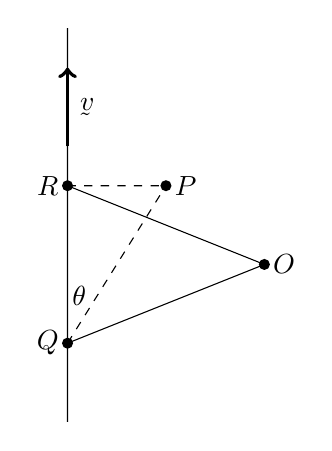
\begin{tikzpicture}

		\draw
		(-2.5,-2) -- (-2.5,3)
		(0,0) -- (-2.5,-1)
		(0,0) -- (-2.5,1);

		\draw[->][line width = 0.5mm]
		(-2.5,1.5) -- (-2.5,2.5);

		\draw[dashed]
		(-2.5,-1) -- (-1.25,1)
		(-2.5,1) -- (-1.25,1);

		\fill[fill=black] (0,0) circle (2pt);
		\fill[fill=black] (-2.5,-1) circle (2pt);
		\fill[fill=black] (-2.5,1) circle (2pt);
		\fill[fill=black] (-1.25,1) circle (2pt);

		\node at (-2.75,-1) {$Q$};
		\node at (-2.75,1) {$R$};
		\node at (0.25,0) {$O$};
		\node at (-1,1) {$P$};
		\node at (-2.25,2) {$\underaccent{\tilde}{v}$};
		\node at (-2.35,-0.4) {$\theta$};

		\end{tikzpicture}


		\end{center}

		From vector addition we have the result $\overrightarrow{OR} = \overrightarrow{OQ} + \overrightarrow{QR}$. Recognising that the required result has the formula for the vector projection of $\overrightarrow{QP}$ in the direction of $\underaccent{\tilde}{v}$, we will examine the rays $\overrightarrow{QP}$ and $\overrightarrow{QR}$.

		\begin{align*}
		\cos{\theta} & = \frac{|\overrightarrow{QR}|}{|\overrightarrow{QP}|}\\
		\therefore |\overrightarrow{QR}| & = |\overrightarrow{QP}|\cos{\theta}\dots\dots\dots\dots\dots(1)\\
		\end{align*}

		Now considering the two rays $\overrightarrow{QP}$ and $\overrightarrow{QR}$, we will determine the value of their dot product, to gain a second equation with $\cos\theta$ as a term.

		\begin{align*}
		\overrightarrow{QP}\cdot{\underaccent{\tilde}{v}} & = |\overrightarrow{QP}||\underaccent{\tilde}{v}|\cos{\theta}\\
		\therefore \cos{\theta} & = \frac{\overrightarrow{QP}\cdot{\underaccent{\tilde}{v}}}{|\overrightarrow{QP}||\underaccent{\tilde}{v}|}\dots\dots\dots\dots\dots(2)\\
		\end{align*}

		Substituting equation $(2)$ into equation $(1)$, we get the following result:

		\begin{align*}
		|\overrightarrow{QR}| & = |\overrightarrow{QP}|\left[\frac{\overrightarrow{QP}\cdot{\underaccent{\tilde}{v}}}{|\overrightarrow{QP}||\underaccent{\tilde}{v}|}\right]\\
		\therefore |\overrightarrow{QR}| & = \frac{\overrightarrow{QP}\cdot{\underaccent{\tilde}{v}}}{|\underaccent{\tilde}{v}|}
		\end{align*}

		We want the vector in the direction of $\underaccent{\tilde}{v}$, yet our current result is only the length of $\overrightarrow{QR}$. In order to get the vector projection in the direction of $\underaccent{\tilde}{v}$, we must multiply our current result for $|\overrightarrow{QR}|$ by the direction of $\underaccent{\tilde}{v}$.

		\begin{align*}
		\therefore |\overrightarrow{QR}| & = \frac{\overrightarrow{QP}\cdot{\underaccent{\tilde}{v}}}{|\underaccent{\tilde}{v}|}\\
		\therefore \overrightarrow{QR} & = \left[\frac{\overrightarrow{QP}\cdot{\underaccent{\tilde}{v}}}{|\underaccent{\tilde}{v}|}\right]\times[\hspace{0.5mm}\hat{\underaccent{\tilde}{v}}\hspace{0.5mm}]\\
		& = \left[\frac{\overrightarrow{QP}\cdot{\underaccent{\tilde}{v}}}{|\underaccent{\tilde}{v}|}\right]\times\left[\frac{\underaccent{\tilde}{v}}{|\underaccent{\tilde}{v}|}\right]\\
		\therefore \overrightarrow{QR} & = \frac{\overrightarrow{QP}\cdot{\underaccent{\tilde}{v}}}{|\underaccent{\tilde}{v}|^2}\underaccent{\tilde}{v}\dots\dots\dots\dots\dots(3)\\
		\end{align*}

		Now using the vector addition equation we derived, $\overrightarrow{OR} = \overrightarrow{OQ} + \overrightarrow{QR}$, and substituting in equation $(3)$, we arrive at the required result.

		\begin{align*}
		\overrightarrow{OR} & = \overrightarrow{OQ} + \overrightarrow{QR}\\
		\therefore \overrightarrow{OR} & = \overrightarrow{OQ} + \frac{\overrightarrow{QP}\cdot{\underaccent{\tilde}{v}}}{|\underaccent{\tilde}{v}|^2}\underaccent{\tilde}{v}\\
		\end{align*}

		\item We are now examining the unit hypercube in $\mathbb{R}^4$, and as a result, are unable to use the cross product, as it is only defined in $\mathbb{R}^3$. As a consequence, we must utilise the above formula that determines the distance between a line and a point, and is defined across $\mathbb{R}^n$, $\forall n \in \mathbb{N}$. 
		\bigbreak
		Similar to the unit cube in $\mathbb{R}^3$, we define each side emanating from the origin, $O(0,0,0,0)$, as a vector, $\underaccent{\tilde}{a}$, $\underaccent{\tilde}{b}$, $\underaccent{\tilde}{c}$, $\underaccent{\tilde}{d}$. These vectors correspond respectively to the unit vectors $\underaccent{\tilde}{i}$, $\underaccent{\tilde}{j}$, $\underaccent{\tilde}{k}$, $\underaccent{\tilde}{l}$. The four axes are $x$, $y$, $z$, $z_1$, where the fourth axis variable will be defined as $z_1$.
		\bigbreak
		For this proof, we will examine the distance from the major diagonal of the hypercube in $\mathbb{R}^4$, to the corner defined by the point $P(1,0,0,0)$. For any point $P$, it can be thought of as a point that contains 4 entries that define its position and are binary values. We will examine the first of two non-trivial cases, where the number of 0s and 1s as position entries that define the point are not equal. Thus any point that satisfies this general form gives the first non-trivial case. As a consequence, we may select any point $P$ that agrees with this criteria, namely $P(1,0,0,0)$. We are able to select any point of the specific general form, as they are all equivalent, as the unit hypercube may be simply rotated about its axes, such that any point can be rotated to any of the other corners. This same property applies in the second non-trivial case.
		\bigbreak
		Now, in order to compute the distance to the major diagonal, we first must determine the direction of the major diagonal. In order to do this, we can visualise the major diagonal of the unit cube in $\mathbb{R}^3$ to be the diagonal on the bottom face of the unit hypercube in $\mathbb{R}^4$. Thus, by vector addition, we get the following result for the major diagonal of the unit hypercube:

		$$
		(\underaccent{\tilde}{a} + \underaccent{\tilde}{b} + \underaccent{\tilde}{c}) + \underaccent{\tilde}{d} = \underaccent{\tilde}{a} + \underaccent{\tilde}{b} + \underaccent{\tilde}{c} + \underaccent{\tilde}{d}
		$$

		Now, examining the formula for the distance between a point and a line, we will use the formula to find the point on the major diagonal of the unit hypercube that is closest to the point $P(1,0,0,0)$. Thus, we need the point $Q$, which will be defined for this proof as $Q(0,0,0,0)$. Furthermore, we need to determine the value of $\overrightarrow{QP}$.

		\begin{align*}
		\overrightarrow{QP} & = P(1,0,0,0) - Q(0,0,0,0)\\
		& = \underaccent{\tilde}{i} - \underaccent{\tilde}{0}\\
		\therefore \overrightarrow{QP} & = \underaccent{\tilde}{i}\\
		\end{align*}

		Furthermore, the major diagonal will be converted into the unit vectors $\underaccent{\tilde}{i}$, $\underaccent{\tilde}{j}$, $\underaccent{\tilde}{k}$, $\underaccent{\tilde}{l}$, for the calculations to follow.

		\begin{align*}
		\underaccent{\tilde}{a} + \underaccent{\tilde}{b} + \underaccent{\tilde}{c} + \underaccent{\tilde}{d} & = \underaccent{\tilde}{i} + \underaccent{\tilde}{j} + \underaccent{\tilde}{k} + \underaccent{\tilde}{l}\\
		\end{align*}

		Now using the formula for the distance between a point $P$ and a line, we can determine the closest point on the line, $R$.

		\begin{align*}
		\overrightarrow{OR} & = \overrightarrow{OQ} + \frac{\overrightarrow{QP}\cdot{\underaccent{\tilde}{v}}}{|\underaccent{\tilde}{v}|^2}\underaccent{\tilde}{v}\\
		& = \underaccent{\tilde}{0} + \frac{(\underaccent{\tilde}{i})\cdot(\underaccent{\tilde}{i} + \underaccent{\tilde}{j} + \underaccent{\tilde}{k} + \underaccent{\tilde}{l})}{|\underaccent{\tilde}{i} + \underaccent{\tilde}{j} + \underaccent{\tilde}{k} + \underaccent{\tilde}{l}|^2}\times(\underaccent{\tilde}{i} + \underaccent{\tilde}{j} + \underaccent{\tilde}{k} + \underaccent{\tilde}{l})\\
		& = \frac{1+0+0+0}{\left(\sqrt{(1)^2 + (1)^2 + (1)^2 + (1)^2}\right)^2}\times(\underaccent{\tilde}{i} + \underaccent{\tilde}{j} + \underaccent{\tilde}{k} + \underaccent{\tilde}{l})\\
		\therefore \overrightarrow{OR} & = \frac{1}{4}(\underaccent{\tilde}{i} + \underaccent{\tilde}{j} + \underaccent{\tilde}{k} + \underaccent{\tilde}{l})\\
		\end{align*}

		This gives the position vector of the point $R$, the closest point on the major diagonal to the point $P$, one of the corners of the hypercube in $\mathbb{R}^4$. Thus $R$ has the coordinates $R(\frac{1}{4},\frac{1}{4},\frac{1}{4},\frac{1}{4})$. Now we will determine the distance between $R$ and $P$.

		\begin{align*}
		\overrightarrow{PR} & = R(\frac{1}{4},\frac{1}{4},\frac{1}{4},\frac{1}{4}) - P(1,0,0,0)\\
		& = \frac{1}{4}\underaccent{\tilde}{i} + \frac{1}{4}\underaccent{\tilde}{j} + \frac{1}{4}\underaccent{\tilde}{k} + \frac{1}{4}\underaccent{\tilde}{l} - \underaccent{\tilde}{i}\\
		\therefore \overrightarrow{PR} & = -\frac{3}{4}\underaccent{\tilde}{i} + \frac{1}{4}\underaccent{\tilde}{j} + \frac{1}{4}\underaccent{\tilde}{k} + \frac{1}{4}\underaccent{\tilde}{l}\\
		\therefore |\overrightarrow{PR}| & = \sqrt{\left(-\frac{3}{4}\right)^2 + \left(\frac{1}{4}\right)^2 + \left(\frac{1}{4}\right)^2 + \left(\frac{1}{4}\right)^2}\\
		\therefore |\overrightarrow{PR}| & = \frac{\sqrt{3}}{2}\\
		\end{align*}

		If we now consider the second non-trivial case, the point can have the same number of 1s and 0s as position entries that define the point. Thus, any point that this general case holds for, gives the same solution. As a result the point $P$ can be chosen as any point that satisifies the crtieria, namely $P(1,1,0,0)$. We now must compute the interval $\overrightarrow{QP}$, which is the same process as above.

		\begin{align*}
		\overrightarrow{QP} & = P(1,1,0,0) - Q(0,0,0,0)\\
		& = \underaccent{\tilde}{i} + \underaccent{\tilde}{j} - \underaccent{\tilde}{0}\\
		\therefore \overrightarrow{QP} & = \underaccent{\tilde}{i} + \underaccent{\tilde}{j}\\
		\end{align*}

		Thus computing the position of point $R$, that is the closest point on the line to the point $P$, we use the same processes as above.

		\begin{align*}
		\overrightarrow{OR} & = \overrightarrow{OQ} + \frac{\overrightarrow{QP}\cdot{\underaccent{\tilde}{v}}}{|\underaccent{\tilde}{v}|^2}\underaccent{\tilde}{v}\\
		& = \underaccent{\tilde}{0} + \frac{(\underaccent{\tilde}{i} + \underaccent{\tilde}{j})\cdot(\underaccent{\tilde}{i} + \underaccent{\tilde}{j} + \underaccent{\tilde}{k} + \underaccent{\tilde}{l})}{|\underaccent{\tilde}{i} + \underaccent{\tilde}{j} + \underaccent{\tilde}{k} + \underaccent{\tilde}{l}|^2}\times(\underaccent{\tilde}{i} + \underaccent{\tilde}{j} + \underaccent{\tilde}{k} + \underaccent{\tilde}{l})\\
		& = \frac{1+1+0+0}{\left(\sqrt{(1)^2 + (1)^2 + (1)^2 + (1)^2}\right)^2}\times(\underaccent{\tilde}{i} + \underaccent{\tilde}{j} + \underaccent{\tilde}{k} + \underaccent{\tilde}{l})\\
		& = \frac{2}{4}(\underaccent{\tilde}{i} + \underaccent{\tilde}{j} + \underaccent{\tilde}{k} + \underaccent{\tilde}{l})\\
		\therefore \overrightarrow{OR} & = \frac{1}{2}(\underaccent{\tilde}{i} + \underaccent{\tilde}{j} + \underaccent{\tilde}{k} + \underaccent{\tilde}{l})\\
		\end{align*}	

		Thus $R$ has the coordinates $R(\frac{1}{2},\frac{1}{2},\frac{1}{2},\frac{1}{2})$. Now we will determine the distance between $R$ and $P$.

		\begin{align*}
		\overrightarrow{PR} & = R(\frac{1}{2},\frac{1}{2},\frac{1}{2},\frac{1}{2}) - P(1,1,0,0)\\
		& = \frac{1}{2}\underaccent{\tilde}{i} + \frac{1}{2}\underaccent{\tilde}{j} + \frac{1}{2}\underaccent{\tilde}{k} + \frac{1}{2}\underaccent{\tilde}{l} - (\underaccent{\tilde}{i} + \underaccent{\tilde}{j})\\
		\therefore \overrightarrow{PR} & = -\frac{1}{2}\underaccent{\tilde}{i} - \frac{1}{2}\underaccent{\tilde}{j} + \frac{1}{2}\underaccent{\tilde}{k} + \frac{1}{2}\underaccent{\tilde}{l}\\
		\therefore |\overrightarrow{PR}| & = \sqrt{\left(-\frac{1}{2}\right)^2 + \left(-\frac{1}{2}\right)^2 + \left(\frac{1}{2}\right)^2 + \left(\frac{1}{2}\right)^2}\\
		\therefore |\overrightarrow{PR}| & = 1\\
		\end{align*}

		The final case to consider is fairly trivial, it is using the point $P$ as either all 1's or all 0's. This results in computing the distance between the major diagonal and the two corners, $P(0,0,0,0)$ and $P(1,1,1,1)$, that are in fact the endpoints of the major diagonal. Thus the distance is clearly zero.
		
		Thus the three cases give the three distances, $\frac{\sqrt{3}}{2}$, $1$ and $0$.


	\end{enumerate}

\end{enumerate}







\end{document}